%% LyX 2.3.7 created this file.  For more info, see http://www.lyx.org/.
%% Do not edit unless you really know what you are doing.
\documentclass[english]{article}
\usepackage{lmodern}
\renewcommand{\sfdefault}{lmss}
\usepackage{courier}
\usepackage[T1]{fontenc}
\usepackage[latin9]{inputenc}
\usepackage{pgfplots}
\usepackage{geometry}
\geometry{verbose,tmargin=0.8in,bmargin=0.8in,lmargin=1in,rmargin=1in,headheight=0cm,headsep=0cm}
\usepackage{babel}
\usepackage{array}
\usepackage[unicode=true]
 {hyperref}

\makeatletter

%%%%%%%%%%%%%%%%%%%%%%%%%%%%%% LyX specific LaTeX commands.
\providecommand{\LyX}{\texorpdfstring%
  {L\kern-.1667em\lower.25em\hbox{Y}\kern-.125emX\@}
  {LyX}}
%% Because html converters don't know tabularnewline
\providecommand{\tabularnewline}{\\}

%%%%%%%%%%%%%%%%%%%%%%%%%%%%%% Textclass specific LaTeX commands.
\newenvironment{lyxcode}
	{\par\begin{list}{}{
		\setlength{\rightmargin}{\leftmargin}
		\setlength{\listparindent}{0pt}% needed for AMS classes
		\raggedright
		\setlength{\itemsep}{0pt}
		\setlength{\parsep}{0pt}
		\normalfont\ttfamily}%
	 \item[]}
	{\end{list}}

\makeatother

\usepackage{listings}
\renewcommand{\lstlistingname}{Listing}

\begin{document}
\begin{center}
{\Large{}CSCE 221 Cover Page\smallskip{}
}{\Large\par}
\par\end{center}

\begin{center}
{\large{}Tianlan~~~~~~~~~~~~~~~~~~Li ~~~~~~~~~~~~~~~~~~~~~532003637~~~~~~~~~~~~~~\bigskip{}
}{\large\par}
\par\end{center}

\begin{center}
{\large{}User Name ~~~~~~~~~~~~~~~~~~~rainsuds@tamu.edu~~~~~~~~~~~~~~~~~~~~~~~~~~~~~~}\medskip{}
\par\end{center}
\begin{quotation}
Please list all sources in the table below including web pages which
you used to solve or implement the current homework. If you fail to
cite sources you can get a lower number of points or even zero, read
more: \href{http://aggiehonor.tamu.edu/}{Aggie Honor System Office}
\medskip{}
\medskip{}
\end{quotation}
\begin{center}
\begin{tabular}{|c|c|c|c|}
\hline 
Type of sources  & ~~~~~~~~~~~~~~~~~~~~~~~~~~~~~ & ~~~~~~~~~~~~~~~~~~~~~~~~~~~~~~~~ & ~~~~~~~~~~~~~~~~~~~~~~~~~~~~~~~~~\tabularnewline
 &  &  & \tabularnewline
 &  &  & \tabularnewline
\hline 
\hline 
People &  &  & \tabularnewline
 &  &  & \tabularnewline
 &  &  & \tabularnewline
\hline 
Web pages (provide URL)  &  &  & \tabularnewline
 &  &  & \tabularnewline
 &  &  & \tabularnewline
\hline 
Printed material &  &  & \tabularnewline
 &  Fourth Edition Data Structures and Algorithm Analysis in C++ &  & \tabularnewline
 &  &  & \tabularnewline
\hline 
Other Sources  &  &  & \tabularnewline
 &  &  & \tabularnewline
 &  &  & \tabularnewline
\hline 
\end{tabular}
\par\end{center}

\medskip{}

\begin{quotation}
I certify that I have listed all the sources that I used to develop
the solutions/codes to the submitted work.

\textquotedblleft \emph{On my honor as an Aggie, I have neither given
nor received any unauthorized help on this academic work.}\textquotedblright{} 
\end{quotation}
\vspace{0.5cm}

\begin{tabular}{cccccc}
Tianlan Li  & ~~~~~~~~~~~~~~~~~~~~~~~~~~~ &  & ~~~~~~~~~~~~~~~~~~~~~ & 9/16/2023  & ~~~~~~~~~~~~~~~~~~~~\tabularnewline
\end{tabular}\vfill{}

\pagebreak{}
\begin{center}
\textbf{\Large{}Homework 1}{\Large\par}
\par\end{center}

\begin{center}
\textbf{\large{}Check the Canvas calendar for the deadliness. }\\
\textbf{\large{}The homework submission to Gradescope only.}{\large\par}
\par\end{center}
\begin{quote}
\textbf{Typeset your solutions to the homework problems listed below
using \LaTeX{} (or \LyX ). See the class webpage for information about
their installation and tutorials.}
\end{quote}
\noindent \begin{flushleft}
\textbf{Homework 1 Objectives:}
\par\end{flushleft}
\begin{enumerate}
\item Developing the C++ programming skills by using
\begin{enumerate}
\item templated dynamic arrays and STL vectors
\item tests for checking correctness of a program.
\end{enumerate}
\item Comparing theory with a computation experiment in order to classify
algorithm.
\item Preparing reports/documents using the professional software \LaTeX{}
or \LyX .
\item Understanding the definition of the big-O asymptotic notation.
\item Classifying algorithms based on pseudocode.
\end{enumerate}
\noindent \begin{flushleft}
\rule[0.5ex]{1\columnwidth}{1pt}
\par\end{flushleft}
\begin{enumerate}
\item (25 points) Include your C++ code in the problem solution\textemdash \textbf{do
not use attachments or screenshots.}
\begin{enumerate}
\item (10 points) Use the STL class \texttt{vector<int>} to write two C++
functions that return true if there exist \textbf{two} elements of
the vector such that their \textbf{product} is divisible by 12, and
return false otherwise. The efficiency of the first function should
be $O(n)$ and the efficiency of second one should be $O(n^{2})$
where $n$ is the size of the vector.
\item[\textbf{Solution 1:}]
\begin{lstlisting}[language={C++},basicstyle={\small\ttfamily},showstringspaces=false]
bool productDivisibleBy12_O_N(const std::vector<int>& nums) {
    int countDivBy2 = 0;
    int countDivBy3 = 0;
    int countDivBy4 = 0;
    int countDivBy6 = 0;
    
    for (int num : nums) {
        if (num % 12 == 0 && nums.size() >= 2)
            return true;
        else if (num % 6 == 0)
            countDivBy6;
        else if (num % 4 == 0)
            countDivBy4++;
        else if (num % 3 == 0)
            countDivBy3++;
        else if (num % 2 == 0)
            countDivBy2++;           
    }
    // 3*4 2*6
    if (countDivBy4 >= 1 && countDivBy3 >= 1)
        return true;
    if (countDivBy2 >= 1 && countDivBy6 >= 1)
        return true;

    return false;
}
\end{lslisting}
\item[\textbf{Solution 2:}]
\begin{lstlisting}[language={C++},basicstyle={\small\ttfamily},showstringspaces=false]
bool productDivisibleBy12_O_N2(const std::vector<int>& nums) {
    int n = nums.size();

    for (int i = 0; i < n; i++) {
        for (int j = i + 1; j < n; j++) {
            if (nums[i] * nums[j] % 12 == 0)
                return true;
        }
    }
    return false;
}
\end{lstlisting}

\item (6 points) Justify your answer by writing the running time functions
in terms of $n$ for both the algorithms and their classification
in terms of big-O asymptotic notation. 
\item[\textbf{Solution:}] 
The $O(n)$ approach is classified as $O(n)$, indicating a linear time complexity. 
The $O(n^{2})$ approach is classified as $O(n^{2})$, indicating a quadratic time complexity.

\item (2 points) What do you consider as an operation for each algorithm? 
\item[\textbf{Solution:}]
In the $O(n)$ approach, operation includes modulus operation, arithmetic operations, and comparison operations. Meanwhile in the $O(n^{2})$ approach, only the comparison operation combined with modulus was used.

\item (2 points) Are the best and worst cases for both the algorithms the
same in terms of big-O notation? Justify your answer. 
\item[\textbf{Solution:}]
For the $O(n)$ algorithm, the best-case scenario for this algorithm occurs when the first elements of the vector is a multiple of 12 and the size of the array is larger than 2, which the function returns true after examining just one elements, so it performs in constant time, O(1). In the worst-case scenario is when none of the pairs of elements in the vector have a product divisible by 12, which the function iterates through all 'n' elements of the vector, performing the constant-time operations during each iteration. Therefore, the worst-case time complexity is $O(n)$. \\
For the $O(n^{2})$ algorithm, best-case scenario for this algorithm is also when the first pair of elements in the vector has a product divisible by 12, which the function returns true after examining just one pair of elements, so it performs in constant time, O(1). In the worst-case scenario occurs when none of the pairs of elements in the vector have a product divisible by 12, which the function needs to compare all possible pairs of 'n' elements in the vector using two nested loops. Therefore, the worst-case time complexity is $O(n^{2})$.

\item (5 points) Describe the situations of getting the best and worst cases,
give the samples of the input for each case, and check if your running
time functions match the number of operations.
\item[\textbf{Solution:}]
For the $O(n)$ algorithm, the best-case scenario for this algorithm can be archieve using vec = \{12, 1\}, which is has $O(1)$ time complexity. Worst case can be archieved by vec = \{1, 2, 3, 5, 7, 9, 11\} which has a size of 7, and the runtime would be O(n) with n = 7. \\
For the $O(n^{2})$ algorithm, best-case scenario can be also archieve by vec = \{12, 1\} with checking 1 pair of combination results in $O(1)$ time complexity. For worst-case, using the same example  vec = \{1, 2, 3, 5, 7, 9, 11\}, the function evaluates all possible combinations which leads to a run-time of $O(n*(n-1)) / 2$, or $O(21)$ operation in this case. 

\vfill{}
\end{enumerate}
\newpage{}
\item (50 points + bonus) The binary search algorithm problem.
\begin{enumerate}
\item (5 points) Implement a templated C++ function for the binary search
algorithm based on the set of the lecture slides\textit{ ``Analysis
of Algorithms''}.

{\small{}}
\begin{lstlisting}[language={C++},basicstyle={\small\ttfamily},showstringspaces=false]
int Binary_Search(vector<int> &v, int x) {
   int mid, low = 0;     
   int high = (int) v.size()-1;     
   while (low < high) {         
      mid = (low+high)/2;                 
      if (num_comp++, v[mid] < x) low = mid+1;         
      else high = mid;     
   }     
   if (num_comp++, x == v[low]) return low; //OK: found          
   return -1; //not found
} 
\end{lstlisting}
{\small\par}
Be sure that before calling \texttt{Binary\_Search}, elements of the
vector \texttt{v} are arranged in \textbf{ascending} order. The function
should also keep track of the number of comparisons used to find the
target \texttt{x}. The (global) variable \texttt{num\_comp} keeps
the number of comparisons and initially should be set to zero. 

\item[\textbf{Solution:}]
\begin{verbatim}
int Binary_Search(std::vector<int> &v, int x, int &num_comp) {
    int mid, low = 0;
    int high = (int) v.size() - 1;
    while (low < high) {
        mid = (low + high) / 2;

        if (num_comp++, v[mid] < x)
            low = mid+1;
        else
            high = mid;
        }
    if (num_comp++, x == v[low]) return low; //OK: found
    return -1; //not found
} 
\end{verbatim}
\medskip{}


\item (10 points) Test your algorithm for correctness using a vector of
data with 16 elements sorted in ascending order. An error message
should be printed or exception should be thrown when the input vector
is unsorted.\\
What is the value of \texttt{num\_comp} in the cases when 
\begin{enumerate}
\item the target \texttt{x} is the first element of the vector \texttt{v}
\begin{verbatim}
v = {1, 2, 3, 4, 5, 6, 7, 8, 9, 10, 11, 12, 13, 14, 15, 16};
Element 1 found at index 0
Number of comparisons: 5
\end{verbatim}
\item the target \texttt{x} is the last element of the vector \texttt{v}
\begin{verbatim}
v = {1, 2, 3, 4, 5, 6, 7, 8, 9, 10, 11, 12, 13, 14, 15, 16};
Element 1 found at index 15
Number of comparisons: 5
\end{verbatim}
\item the target \texttt{x} is in the middle of the vector \texttt{v}
\begin{verbatim}
v = {1, 2, 3, 4, 5, 6, 7, 8, 9, 10, 11, 12, 13, 14, 15, 16};
Element 8 found at index 7
Number of comparisons: 5
\end{verbatim}
\end{enumerate}
What is your conclusion from the testing for $n=16$?\medskip{}
\item[\textbf{Solution:}]
In the best-case, run time for n = 16 is $O(1)$. Worst case is $O(log n)$, or $O(log 16)$

\item (10 points) Test your program using vectors of size $n=2^{k}$ where
$k=0,\,1,2,\dots,11$ populated with consecutive increasing integers
in these ranges: $1,\,2,\,4,\,8,\,16,\,32,\,64,\,128,\,256,\,512,\,1024,\,2048$.
Select the target as the last element in the vector. Record the value
of \texttt{num\_comp} for each vector size in the table below. 

\textbf{}%
\begin{tabular}{|>{\centering}p{2cm}|c|c|}
\hline 
Range {[}1,$n${]} & \multicolumn{1}{>{\centering}p{2cm}|}{Target } & \multicolumn{1}{>{\centering}p{2cm}|}{num\_comp}\tabularnewline
\hline 
\hline 
{[}1, 1{]} & 1 & 1\tabularnewline
\hline 
{[}1, 2{]} & 2 & 2\tabularnewline
\hline 
{[}1, 4{]} & 4 & 3\tabularnewline
\hline 
{[}1, 8{]} & 8 & 4\tabularnewline
\hline 
{[}1, 16{]} & 16 & 5\tabularnewline
\hline 
{[}1, 32{]} & 32 & 6\tabularnewline
\hline 
{[}1, 64{]} & 64 & 7\tabularnewline
\hline 
{[}1, 128{]} & 128 & 8\tabularnewline
\hline 
{[}1, 256{]} & 256 & 9\tabularnewline
\hline 
{[}1, 512{]} & 512 & 10\tabularnewline
\hline 
{[}1, 1024{]} & 1024 & 11\tabularnewline
\hline 
{[}1, 2048{]} & 2048 & 12\tabularnewline
\hline 
\end{tabular}
\item (5 points) Plot the number of comparisons for the vector size $n=2^{k}$,
$k=0,1,2,\dots,11$. You can use a spreadsheet or any graphical package.

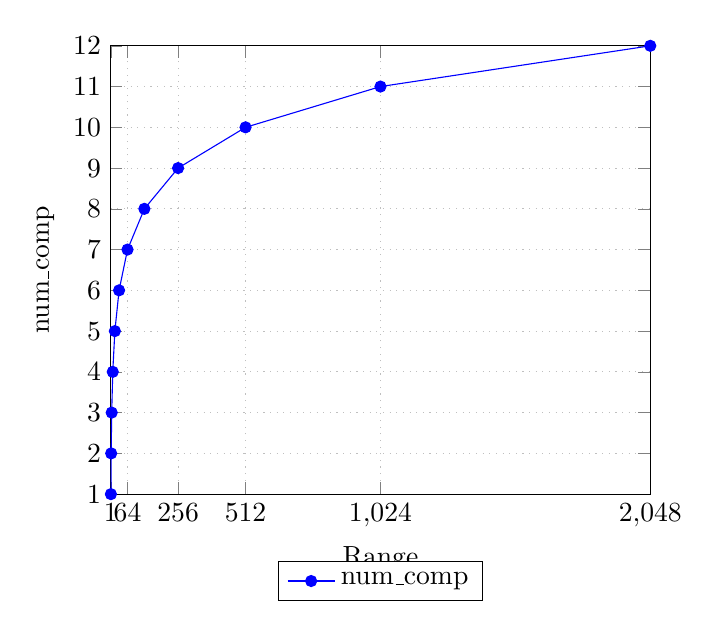
\begin{tikzpicture}
\begin{axis}[
    xlabel={Range},
    ylabel={num\_comp},
    xmin=0, xmax=2048,
    ymin=1, ymax=12,
    xtick={1,64,256,512,1024,2048},
    ytick={1,2,3,4,5,6,7,8,9,10,11,12},
    legend style={at={(0.5,-0.15)},anchor=north},
    grid=both,
    grid style={dotted},
]

\addplot[
    color=blue,
    mark=*,
    ] coordinates {
    (1,1)
    (2,2)
    (4,3)
    (8,4)
    (16,5)
    (32,6)
    (64,7)
    (128,8)
    (256,9)
    (512,10)
    (1024,11)
    (2048,12)
};

\legend{num\_comp}
\end{axis}
\end{tikzpicture}
\medskip{}
\item (5 points) Provide a mathematical formula/function which takes $n$
as an argument, where $n$ is the vector size, and returns as its
value the number of comparisons. Does your formula match the computed
output for any input? Justify your answer.\medskip{}
\item[\textbf{Solution:}]
$ num_comp = \log_{2}(n) + 1$
Yes, the formula matches the computed output for any input since running the code with a sorted\_vector of size 1048576 only uses 21 comparisons, which matches the result using the calculated formula.

\item (5 points) How can you modify your formula/function if the largest
number in a vector is not the exact power of two? Test your program
using input in ranges from $1$ to $n=2^{k}-1$, $k=0,1,2,\dots,11$
and plot the number of comparisons vs. the size of the vector.
\item[\textbf{Solution:}]


\textbf{}%
\begin{tabular}{|c|c|c|}
\hline 
\multicolumn{1}{|c|}{Range {[}1,$n${]}} & \multicolumn{1}{>{\centering}p{2cm}|}{Target } & \multicolumn{1}{>{\centering}p{2cm}|}{num\_comp }\tabularnewline
\hline 
\hline 
{[}1, 1{]} & 1 & 1\tabularnewline
\hline 
{[}1, 3{]} & 3 & 2\tabularnewline
\hline 
{[}1, 7{]} & 7 & 3\tabularnewline
\hline 
{[}1, 15{]} & 15 & 4\tabularnewline
\hline 
{[}1, 31{]} & 31 & 5\tabularnewline
\hline 
{[}1, 63{]} & 63 & 6\tabularnewline
\hline 
{[}1, 127{]} & 127 & 7\tabularnewline
\hline 
{[}1, 255{]} & 255 & 8\tabularnewline
\hline 
{[}1, 511{]} & 511 & 9\tabularnewline
\hline 
{[}1, 1023{]} & 1023 & 10\tabularnewline
\hline 
{[}1, 2047{]} & 2047 & 11\tabularnewline
\hline 
\end{tabular}
\item (5 points) Do you think the number of comparisons in the experiment
above are the same for a vector of strings or a vector of doubles?
Justify your answer.\medskip{}
\item[\textbf{Solution:}]
No, it will not be the same for a vector of strings or doubles since those 2 data structures are not in constant-time operation. Strings sorting will entirely depends on the length of strings and size of the vector, doubles are floating point decimals which are entirely based on the order of sorting. Therefore the number of operations would not be the same.

\item (5 points) Use the big-O asymptotic notation to classify binary search
algorithm and justify your answer.\medskip{}
\item[\textbf{Solution:}]
The binary search algorithm is classified as having a time complexity of O(log n), where "n" is the number of elements in the sorted array.
The basis is to halve the Search Space, thefore causing a logarithmic growth in the number of comparisons as the n increases, and it efficiently divides the search space in half with each iteration. This classification is justified by the algorithm's behavior and its worst-case performance.

\item (Bonus 10 points) Read the sections 1.6.3 and 1.6.4 from the textbook
and modify the algorithm using a functional object to compare vector
elements. How can you modify the binary search algorithm to handle
the vector of descending elements? What will be the value of \texttt{num\_comp}?
Repeat the search experiment for the smallest number in the integer
arrays. Tabulate the results and write a conclusion of the experiment
with your justification. \medskip{}

\begin{tabular}{|>{\centering}p{2cm}|c|c|}
\hline 
Range {[}1,$n${]} & \multicolumn{1}{>{\centering}p{2cm}|}{Target } & \multicolumn{1}{>{\centering}p{2cm}|}{num\_comp}\tabularnewline
\hline 
\hline 
{[}1, 1{]} & 1 & 1\tabularnewline
\hline 
{[}2, 1{]} & 1 & 2\tabularnewline
\hline 
{[}4, 1{]} & 1 & 3\tabularnewline
\hline 
{[}8, 1{]} & 1 & 4\tabularnewline
\hline 
{[}16, 1{]} & 1 & 5\tabularnewline
\hline 
{[}32, 1{]} & 1 & 6\tabularnewline
\hline 
{[}64, 1{]} & 1 & 7\tabularnewline
\hline 
{[}128, 1{]} & 1 & 8\tabularnewline
\hline 
{[}256, 1{]} & 1 & 9\tabularnewline
\hline 
{[}512, 1{]} & 1 & 10\tabularnewline
\hline 
{[}1024, 1{]} & 1 & 11\tabularnewline
\hline 
{[}2048, 1{]} & 1 & 12\tabularnewline
\hline 
\end{tabular}
\item[\textbf{Solution:}]
Despite the descending order, the number of comparisons remains consistent with the worst-case time complexity of O(log n). This is because the binary search algorithm effectively divides the search space by half in each step, regardless of the order of elements.

\newpage{}
\end{enumerate}
\item (25 points) Find running time functions for the algorithms below and
write their classification using big-O asymptotic notation in terms
of $n$. A running time function should provide a formula on the number
of arithmetic operations and assignments performed on the variables
$s$, $t$, or $c$. Note that array indices start from $0$.
\begin{enumerate}
\item \textbf{\small{}Algorithm Ex1(A):}{\small\par}
\begin{lyxcode}
\textbf{\small{}~~Input}{\small{}:~An~array~A~storing~$n\geq1$~integers.}{\small\par}

\textbf{\small{}~~Output}{\small{}:~The~sum~of~the~elements~in~A.}{\small\par}

{\small{}$s\leftarrow A[0]$}{\small\par}

\textbf{\small{}for}{\small{}~$i\leftarrow1$~to~$n-1$~}\textbf{\small{}do}{\small\par}

{\small{}~~~$s\leftarrow s+A[i]$}{\small\par}

\textbf{\small{}end~for}{\small\par}

\textbf{\small{}return}{\small{}~$s$}
\end{lyxcode}
\item[\textbf{Solution:}]
The function has a running time of $O(n)$. The function is excuted $O(1 + (n - 1))$ iterations on s. \vfill{}

\item \textbf{\small{}Algorithm Ex2(A):}{\small\par}
\begin{lyxcode}
\textbf{\small{}~~Input}{\small{}:~An~array~A~storing~$n\geq1$~integers.}{\small\par}

\textbf{\small{}~~Output}{\small{}:~The~sum~of~the~elements~at~even~positions~in~A.}{\small\par}

{\small{}$s\leftarrow A[0]$}{\small\par}

\textbf{\small{}for}{\small{}~$i\leftarrow2$~}\textbf{\small{}to}{\small{}~$n-1$~}\textbf{\small{}by~}{\small{}increments~of~2}\textbf{\small{}~do}{\small\par}

{\small{}~~$s\leftarrow s+A[i]$}{\small\par}

\textbf{\small{}end~for}{\small\par}

\textbf{\small{}return}{\small{}~$s$}
\end{lyxcode}
\item[\textbf{Solution:}]
The function has a running time of $O(n / 2)$. The function is excuted $O(1 + ((n - 2) / 2)$ iterations on s. \vfill{}

\item \textbf{\small{}Algorithm Ex3(A):}{\small\par}
\begin{lyxcode}
{\small{}~~~}\textbf{\small{}Input}{\small{}:~An~array~A~storing~$n\geq1$~integers.}{\small\par}

\textbf{\small{}~~~Output}{\small{}:~The~sum~of~the~partial~sums~in~A.}{\small\par}

{\small{}$s\leftarrow0$}{\small\par}

\textbf{\small{}for}{\small{}~$i\leftarrow0$~~}\textbf{\small{}to}{\small{}~$n-1$~}\textbf{\small{}do}{\small\par}

{\small{}~~~$s\leftarrow s+A[0]$}{\small\par}

\textbf{\small{}~~~for}{\small{}~$j\leftarrow1$~}\textbf{\small{}to}{\small{}~$i$~}\textbf{\small{}do}{\small\par}

{\small{}~~~~~$s\leftarrow s+A[j]$}{\small\par}

{\small{}~~~}\textbf{\small{}end~for}{\small\par}

\textbf{\small{}end~for}{\small\par}
\begin{lyxcode}
\textbf{\small{}return}{\small{}~$s$}
\pagebreak{}
\end{lyxcode}
\item[\textbf{Solution:}]
The function has a running time of $O(n^{2})$. The function is excuted $O((n - 1) * (n - 1))$ iterations on s.\vfill{}

\end{lyxcode}
\item \textbf{\small{}Algorithm Ex4(A):}{\small\par}
\begin{lyxcode}
{\small{}~~~}\textbf{\small{}Input}{\small{}:~An~array~A~storing~$n\geq1$~integers.}{\small\par}

\textbf{\small{}~~~Output}{\small{}:~The~sum~of~the~partial~sums~in~A.}{\small\par}

{\small{}$t\leftarrow A[0]$}{\small\par}

{\small{}$s\leftarrow A[0]$}{\small\par}

\textbf{\small{}for}{\small{}~$i\leftarrow1$~}\textbf{\small{}to}{\small{}~$n-1$~}\textbf{\small{}do}{\small{}~}{\small\par}

{\small{}~~~$s\leftarrow s+A[i]$}{\small\par}

{\small{}~~~$t\leftarrow t+s$}{\small\par}

\textbf{\small{}end~for}{\small\par}

\textbf{\small{}return}{\small{}~$t$}
\end{lyxcode}
\item[\textbf{Solution:}]
The function has a running time of $O(n)$. The function is excuted $O(1 + (2n - 1))$ iterations on s and t. \vfill{}

\item \textbf{\small{}Algorithm Ex5(A, B):}{\small\par}
\begin{lyxcode}
{\small{}~~~}\textbf{\small{}Input}{\small{}:~Arrays~A~and~B~storing~$n\geq1$~integers.}{\small\par}

\textbf{\small{}~~~Output}{\small{}:~The~number~of~elements~in~B~equal~to~the~partial~sums~in~A.}{\small\par}

{\small{}$c\leftarrow0$~//counter}{\small\par}

\textbf{\small{}for}{\small{}~$i\leftarrow0$~}\textbf{\small{}to}{\small{}~$n-1$~}\textbf{\small{}do}{\small{}~}{\small\par}

{\small{}~~~$s\leftarrow0$~//}\emph{\small{}partial~sum}{\small\par}

\textbf{\small{}~~~for}{\small{}~$j\leftarrow0$~}\textbf{\small{}to}{\small{}~$n-1$~}\textbf{\small{}do}{\small\par}

{\small{}~~~~~~$s\leftarrow s+A[0]$}{\small\par}

\textbf{\small{}~~~~~~for}{\small{}~$k\leftarrow1$~}\textbf{\small{}to}{\small{}~$j$~}\textbf{\small{}do}{\small\par}

{\small{}~~~~~~~~~$s\leftarrow s+A[k]$}{\small\par}

{\small{}~~~~~~}\textbf{\small{}end~for}{\small\par}

{\small{}~~~}\textbf{\small{}end~for}{\small\par}

{\small{}~~~}\textbf{\small{}if}{\small{}~$B[i]=s$~}\textbf{\small{}then}{\small\par}

{\small{}~~~~~~$c\leftarrow c+1$}{\small\par}

{\small{}~~~}\textbf{\small{}end~if}{\small\par}

\textbf{\small{}end~for}{\small\par}

\textbf{\small{}return}{\small{}~$c$}
\end{lyxcode}
\item[\textbf{Solution:}]
The function has a running time of $O(n^{3})$. The function is excuted $O(1 + (n - 1))$ iterations on c and $O(n * (n * (n - 1)))$ iterations on s. \vfill{}

\end{enumerate}
\end{enumerate}

\end{document}
